%% Exemplo de utilizacao do estilo de formatacao normas-utf-tex (http://normas-utf-tex.sourceforge.net)
%% dúvidas acessar o site acima
%%
%%
%% Autores: (200?-2011) Hugo Vieira Neto (hvieir@utfpr.edu.br)
%%          (200?-2011) Diogo Rosa Kuiaski (diogo.kuiaski@gmail.com)
%%          (2011-2017) Marcos Talau <talau@users.sourceforge.net>
%% Colaborador:
%%          (2011) César M. Vargas Benitez <cesarvargasb@gmail.com>

%%
%% IMPORTANTE: O texto está escrito com acentuação antiga, atualmente você
%%             pode escrever acentos sem precisar de códigos para tal.
%%

\documentclass[openright]{normas-utf-tex} %openright = o capitulo comeca sempre em paginas impares
%\documentclass[oneside]{normas-utf-tex} %oneside = para dissertacoes com numero de paginas menor que 100 (apenas frente da folha) 

% force A4 paper format
\special{papersize=210mm,297mm}

\usepackage[alf,abnt-emphasize=bf,bibjustif,recuo=0cm, abnt-etal-cite=2, abnt-etal-list=99]{abntcite} %configuracao correta das referencias bibliograficas.

\usepackage[brazil]{babel} % pacote portugues brasileiro
\usepackage[utf8]{inputenc} % pacote para acentuacao direta
\usepackage{amsmath,amsfonts,amssymb} % pacote matematico
\usepackage{graphicx} % pacote grafico
\usepackage{times} % fonte times
\usepackage[final]{pdfpages} % adicao da ata

%Podem utilizar GEOMETRY{...} para realizar pequenos ajustes das margens. Onde, left=esquerda, right=direita, top=superior, bottom=inferior. P.ex.:
%\geometry{left=3.0cm,right=1.5cm,top=4cm,bottom=1cm} 

% ---------- Preambulo ----------
\instituicao{Universidade Tecnológica Federal do Paraná} % nome da instituicao
\programa{Programa de Pós-graduação em Engenharia Elétrica e Informática Industrial} % nome do programa
\area{Informática Industrial} % [Engenharia Biom\'edica] ou [Inform\'atica Industrial] ou [Telem\'atica]

\documento{Dissertação} % [Disserta\c{c}\~ao] ou [Tese]
\nivel{Pos-graduação} % [Mestrado] ou [Doutorado]
\titulacao{Especialista} % [Mestre] ou [Doutor]

\titulo{{Sistema autonomo de gerenciamento de luzes}} % titulo do trabalho em portugues
\title{\MakeUppercase{Self-contained lighting management system}} % titulo do trabalho em ingles

\autor{Luis Denis Pliskievski de Lara} % autor do trabalho
\cita{LARA, Luis Denis Pliskievski de} % sobrenome (maiusculas), nome do autor do trabalho

\palavraschave{IOT, nodeMCU, ESP8266, energia, controle, autonomo} % palavras-chave do trabalho
\keywords{IOT, nomeMCU, ESP8266, energy, contro, self-contained} % palavras-chave do trabalho em ingles

\comentario{\UTFPRdocumentodata\ apresentada ao \UTFPRprogramadata\ da \ABNTinstituicaodata\ como requisito parcial para obtenção do grau de ``\UTFPRtitulacaodata\ em Ciências'' -- Área de Concentração: \UTFPRareadata.}

    \orientador{Glauber Brante} % nome do orientador do trabalho
%\orientador[Orientadora:]{Nome da Orientadora} % <- no caso de orientadora, usar esta sintaxe
%\coorientador{Nome do Co-orientador} % nome do co-orientador do trabalho, caso exista
%\coorientador[Co-orientadora:]{Nome da Co-orientadora} % <- no caso de co-orientadora, usar esta sintaxe
%\coorientador[Co-orientadores:]{Nome do Co-orientador} % no caso de 2 co-orientadores, usar esta sintaxe
%\coorientadorb{Nome do Co-orientador 2}	% este comando inclui o nome do 2o co-orientador

\local{Curitiba} % cidade
\data{\the\year} % ano automatico

% desativa hifenizacao mantendo o texto justificado.
% thanks to Emilio C. G. Wille
\tolerance=1
\emergencystretch=\maxdimen
\hyphenpenalty=10000
\hbadness=10000
\sloppy

%---------- Inicio do Documento ----------
\begin{document}

\capa % geracao automatica da capa
\folhaderosto % geracao automatica da folha de rosto

% Lembre-se de que a ficha catalografica eh impressa no verso da folha de rosto
% Ficha catalografica
\fichacatpum{T137}
\fichacatautor{Lara, Luis Denis Pliskievski de}
\fichacatpgbib{\pageref{bibstart}-\pageref{bibend}}
\fichacatpalcha{1. Teoria do controle. 2. Redes de comutação. 3. TCP/IP (Protocolo de rede de computação), ...}
\fichacatpdois{CDD (22. ed.) 621.3}
\fichacatbib{Biblioteca xxxxxx}
\fichacat

% insercao da ATA
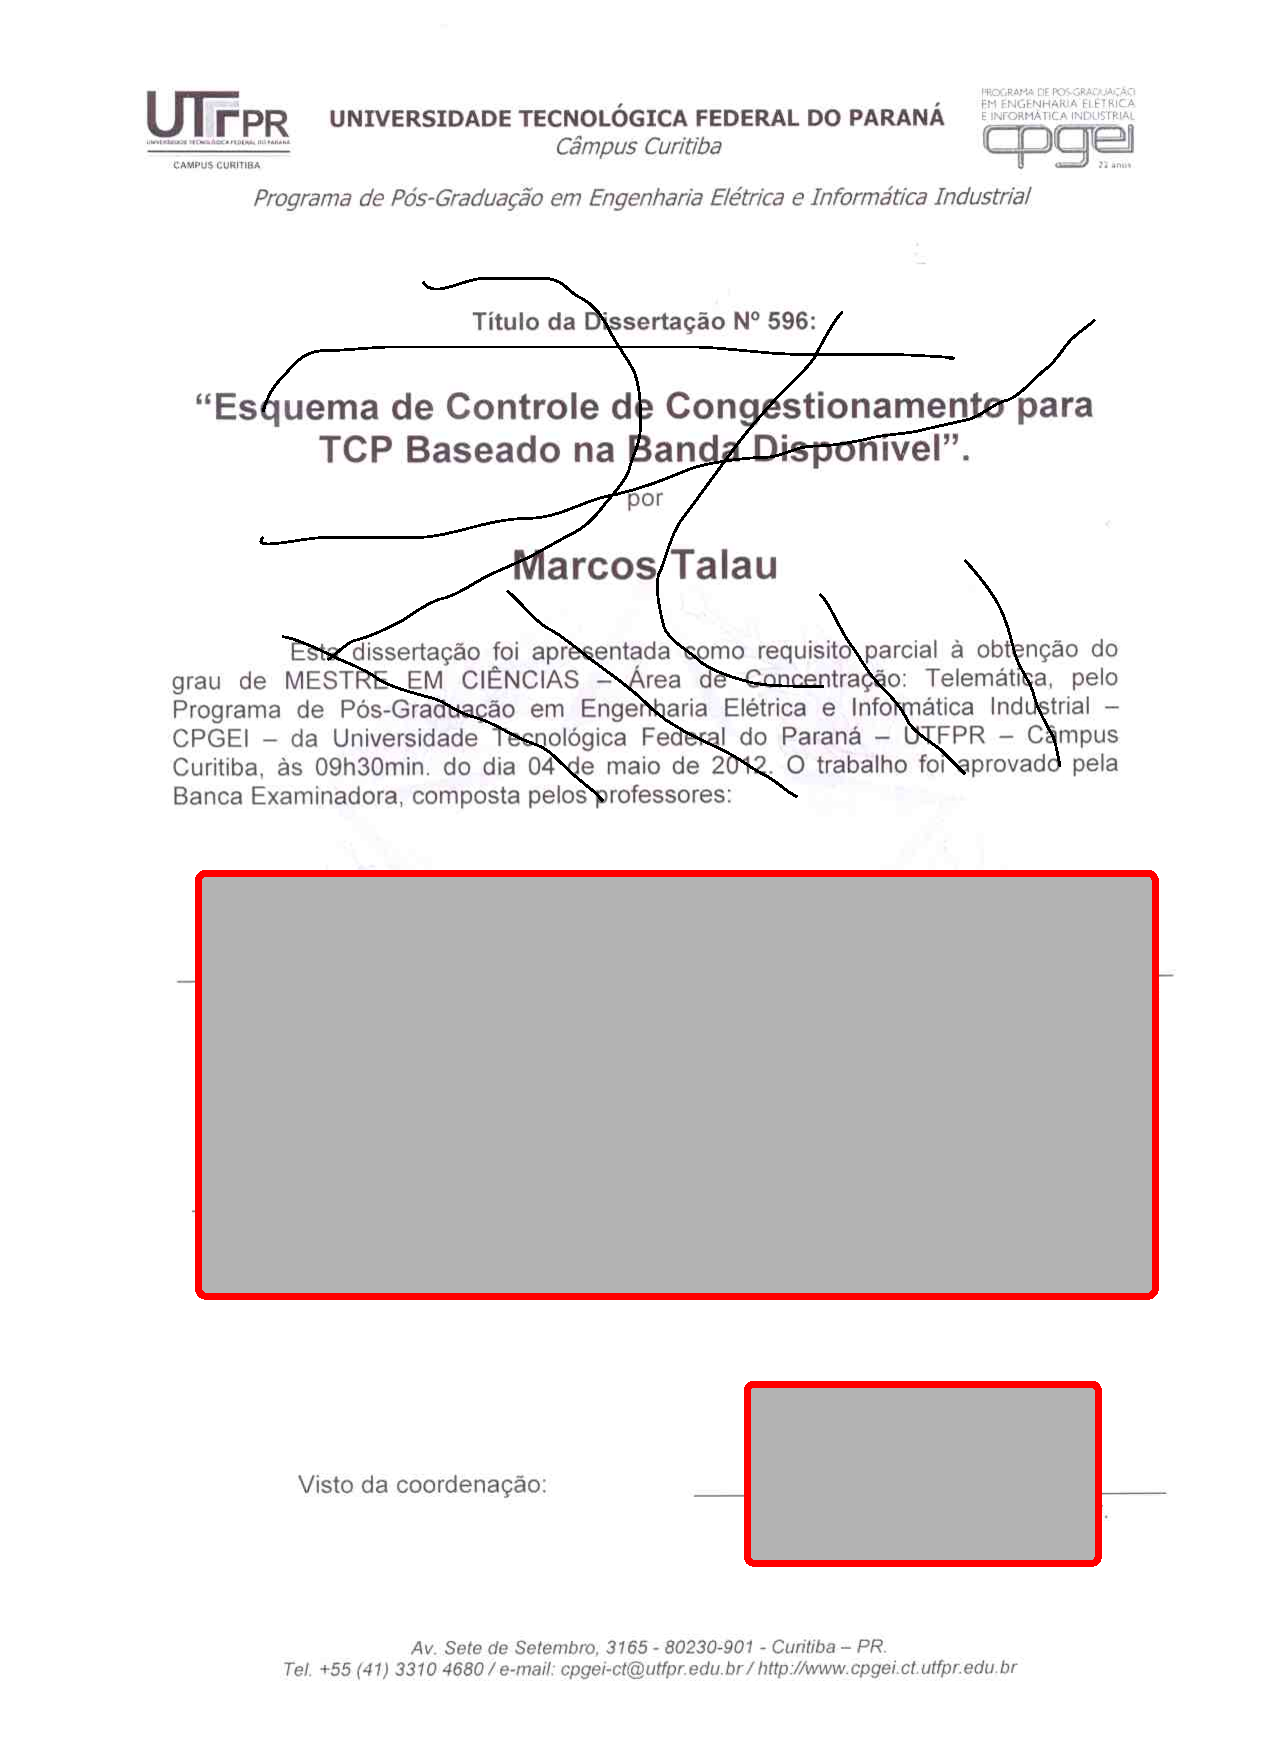
\includepdf{ata.pdf}

% dedicatoria
\begin{dedicatoria}
Texto da dedicat\'oria.
\end{dedicatoria}

% agradecimentos (opcional)
\begin{agradecimentos}
Texto dos agradecimentos.
\end{agradecimentos}

% epigrafe (opcional)
\begin{epigrafe}
Texto da ep\'igrafe.
\end{epigrafe}

%resumo
\begin{resumo}
Texto do resumo (m\'aximo de 500 palavras).
\end{resumo}

%abstract
\begin{abstract}
Abstract text (maximum of 500 words).
\end{abstract}

% listas (opcionais, mas recomenda-se a partir de 5 elementos)
\listadefiguras % geracao automatica da lista de figuras
\listadetabelas % geracao automatica da lista de tabelas
\listadequadros % adivinhe :)
\listadesiglas % geracao automatica da lista de siglas
\listadesimbolos % geracao automatica da lista de simbolos

% sumario
\sumario % geracao automatica do sumario


%---------- Inicio do Texto ----------
% recomenda-se a escrita de cada capitulo em um arquivo texto separado (exemplo: intro.tex, fund.tex, exper.tex, concl.tex, etc.) e a posterior inclusao dos mesmos no mestre do documento utilizando o comando \input{}, da seguinte forma:
%\input{intro.tex}
%\input{fund.tex}
%\input{exper.tex}
%\input{concl.tex}

\setcounter{page}{12}

%---------- Primeiro Capitulo ----------
\chapter{Introdução}

Com o advento da internet e evolução, temos a possibilidade de criar dispositivos inteligentes para nos auxiliar em situações corriqueiras, como controle de acesso, controle de frotas, gerenciamento de energia e água.

Nesse trabalho iremos desmostrar um sistema inteliganete de gerenciamento de luzes para comercio, empresas e mesmo casas.

Para o desenvolvimento do recurso usaremos os itens:

\begin{itemize}
       	\item ESP8266 - NomeMCU V3
        \item Sensor de corrente Allegro ACS712 (ACS712ELCTR-30A-)
        \item Servidor MQTT
        \item Sensor de presença PIR DYP-ME003
\end{itemize}
\section{Motivação}

Há um grande disperdício de energia em corporações e lojas devido  a falta de controle sobre o consumo de energia o que em analise calculista pode representar um impacto as contas da empresa e ao meio ambiente, pois hoje falamos muito em eficiente energética e isso pode trazer efeitos signiticativos para administração das empresas.

\section{Objetivos}

\subsection{Objetivo Geral}

O objetivo prinicipal é demonstrar e gerenciar o consumo de energia sobre fontes de iluminação visando diminuir o consumo e aumentar a eficiência do uso dos recursos energéticos. 

\subsection{Objetivos Específicos}

\begin{itemize}
	\item Controlar o consumo de energia.
	\item Representar por meio de números o consumo real. 
	\item Melhorar o consumo energético através de gerenciamento autonomo.
	\item Entregar uma previsão de consumo x gasto mensal.
\end{itemize}


%---------- Segundo Capitulo ----------
\chapter{Desenvolvimento}
\label{chap:desenv}
 
Para o desenvolvimento do projeto foi utilizando a linguagem python, suportada pelo módulo ESP8266 além de C++.

Durente o processo de desenvolvimento previmos a nomeação do módulo durante a primeira inicialização, após a configuração do SSID e senha da rede.

Com a rede configurada o nó começa a enviar dados da para um servidor MQTT para ser tratado no painel de gerenciamento. 

\subsection{NodeMCU}
Optei pelo uso do microcontrolador ESP8266, presente no módulo NODEMCU, que possui as seguites caracteristas:
\begin{itemize}
    \item Certificação WIFI Alliance;
    \item Protocolos 802.11 b/g/n;
    \item CPU Tensilica L106 32-bit processor (80MHz ~ 160MHz );
    \item 4MB de armazenamento;
    \item Suporte aos modos Station/SoftAP/SoftAP+Station;
    \item Autenticação WPA/WPA2 com encriptação WEP/TKIP/AES;
    \item Supoter atualização OTA;
    \item Procolocolos de Rede IPv4, TCP/UDP/HTTP;
\end{itemize}

Durante o processo de desenvolvimento do projeto foi encontrado uma limitação do uso de vários nós em rede MASH, pois há um limite de conexões simultaneas permitidas, ou seja se mais 5 nós tentarem se manter conectados a um NodeMCU a conexão mais antiga será derrubada, podendo gerar assim algumas falhas de tramissão de dados. 

Pois isso optei em não usar a rede MASH e manter todos os nós comunicando diretamente com o servidor MQTT.

Caso a rede esteja indisponível por alguma motivo o nó poderá armazenar informações em sua memória de até 7 dias.

\subsection{Sensor de corrente Allegro ACS712}
O medidor de corrente Allegro ACS712 pode trabalhar com correntes de -30A à +30A amperes, mais que suficiente para os padrões que usamos em estrutura de iluminação, aonde as correntes geralmente não são maiores que 10A.

A taxa de amostragem durante o desenvolvimento deve um pequena diferença comparando com o resultado de multimetro. Essa diferença ficou entre 55mA e 70mA. Isso acontece devido ao ruído do L106 e o ruído do próprio Allegro ACS712.

Para calular o consumo utilizamos algumas informações do padrão brasileiro, como a taxa de amostragem de 60Hz de nossas redes. Com base nessas informações e utilizando a biblioteca EmonLib, a biblioteca originalmente foi desenvolvida para Arduíno mas é compatível com o ESP8266 utilizado.

Uma vez realizada a medição os dados são enviados via MQTT para serem exibidos no front-end.

\subsection{Sensor de presença PIR DYP-ME003}

Também utilizamos um sensor de presença para ter um controle automatico de uso de salas, 

Com isso no momento que a pessoa entra da sala o sensor envia um sinal que acende as lampadas automaticamente e começa a bilhetagem das luzes naquela sala.


%---------- Terceiro Capitulo ----------
\chapter{Conclusão}

Espera-se que o uso do estilo de formata\c{c}\~ao \LaTeX\ adequado \`as Normas para Elabora\c{c}\~ao de Trabalhos Acad\^emicos da UTFPR ({\ttfamily normas-utf-tex.cls}) facilite a escrita de documentos no \^ambito desta institui\c{c}\~ao e aumente a produtividade de seus autores. Para usu\'arios iniciantes em \LaTeX, al\'em da bibliografia especializada j\'a citada, existe ainda uma s\'erie de recursos~\cite{CTAN2009} e fontes de informa\c{c}\~ao~\cite{TeX-Br2009,Wikibooks2009} dispon\'iveis na Internet.

Recomenda-se o editor de textos Kile como ferramenta de composi\c{c}\~ao de documentos em \LaTeX\ para usu\'arios Linux. Para usu\'arios Windows recomenda-se o editor \TeX nicCenter~\cite{TeXnicCenter2009}. O \LaTeX\ normalmente j\'a faz parte da maioria das distribui\c{c}\~oes Linux, mas no sistema operacional Windows \'e necess\'ario instalar o software \textsc{MiK}\TeX~\cite{MiKTeX2009}.

Al\'em disso, recomenda-se o uso de um gerenciador de refer\^encias como o JabRef~\cite{JabRef2009} ou Mendeley~\cite{Mendeley2009} para a cataloga\c{c}\~ao bibliogr\'afica em um arquivo \textsc{Bib}\TeX, de forma a facilitar cita\c{c}\~oes atrav\'es do comando {\ttfamily \textbackslash cite\{\}} e outros comandos correlatos do pacote \textsc{abn}\TeX. A lista de refer\^encias deste documento foi gerada automaticamente pelo software \LaTeX\ + \textsc{Bib}\TeX\ a partir do arquivo {\ttfamily reflatex.bib}, que por sua vez foi composto com o gerenciador de refer\^encias JabRef.

O estilo de formata\c{c}\~ao \LaTeX\ da UTFPR e este exemplo de utiliza\c{c}\~ao foram elaborados por Diogo Rosa Kuiaski (diogo.kuiaski@gmail.com) e Hugo Vieira Neto (hvieir@utfpr.edu.br), com contribui\c{c}\~oes de C\'esar Vargas Benitez. Sugest\~oes de melhorias s\~ao bem-vindas.


%---------- Referencias ----------
\clearpage % this is need for add +1 to pageref of bibstart used in 'ficha catalografica'.
\label{bibstart}
\bibliography{reflatex} % geracao automatica das referencias a partir do arquivo reflatex.bib
\label{bibend}

%---------- Apendices (opcionais) ----------
\apendice
\chapter{Nome do Ap\^endice}

Use o comando {\ttfamily \textbackslash apendice} e depois comandos {\ttfamily \textbackslash chapter\{\}}
para gerar t\'itulos de ap\^en-dices.


% ---------- Anexos (opcionais) ----------
\anexo
\chapter{Nome do Anexo}

Use o comando {\ttfamily \textbackslash anexo} e depois comandos {\ttfamily \textbackslash chapter\{\}}
para gerar t\'itulos de anexos.


% --------- Ordenacao Afabetica da Lista de siglas --------
%\textbf{* Observa\c{c}\~oes:} a ordenacao alfabetica da lista de siglas ainda nao eh realizada de forma automatica, porem
% eh possivel se de realizar isto manualmente. Duas formas:
%
% ** Primeira forma)
%    A ordenacao eh feita com o auxilio do comando 'sort', disponivel em qualquer
% sistema Linux e UNIX, e tambem em sistemas Windows se instalado o coreutils (http://gnuwin32.sourceforge.net/packages/coreutils.htm)
% comandos para compilar e ordenar, supondo que seu arquivo se chame 'dissertacao.tex':
%
%      $ latex dissertacao
%      $ bibtex dissertacao && latex dissertacao
%      $ latex dissertacao
%      $ sort dissertacao.lsg > dissertacao.lsg.tmp
%      $ mv dissertacao.lsg.tmp dissertacao.lsg
%      $ latex dissertacao
%      $ dvipdf dissertacao.dvi
%
%
% ** Segunda forma)
%\textbf{Sugest\~ao:} crie outro arquivo .tex para siglas e utilize o comando \sigla{sigla}{descri\c{c}\~ao}.
%Para incluir este arquivo no final do arquivo, utilize o comando \input{arquivo.tex}.
%Assim, Todas as siglas serao geradas na ultima pagina. Entao, devera excluir a ultima pagina da versao final do arquivo
% PDF do seu documento.


%-------- Citacoes ---------
% - Utilize o comando \citeonline{...} para citacoes com o seguinte formato: Autor et al. (2011).
% Este tipo de formato eh utilizado no comeco do paragrafo. P.ex.: \citeonline{autor2011}

% - Utilize o comando \cite{...} para citacoeses no meio ou final do paragrafo. P.ex.: \cite{autor2011}



%-------- Titulos com nomes cientificos (titulo, capitulos e secoes) ----------
% Regra para escrita de nomes cientificos:
% Os nomes devem ser escritos em italico, 
%a primeira letra do primeiro nome deve ser em maiusculo e o restante em minusculo (inclusive a primeira letra do segundo nome).
% VEJA os exemplos abaixo.
% 
% 1) voce nao quer que a secao fique com uppercase (caixa alta) automaticamente:
%\section[nouppercase]{\MakeUppercase{Estudo dos efeitos da radiacao ultravioleta C e TFD em celulas de} {\textit{Saccharomyces boulardii}}
%
% 2) por padrao os cases (maiusculas/minuscula) sao ajustados automaticamente, voce nao precisa usar makeuppercase e afins.
% \section{Introducao} % a introducao sera posta no texto como INTRODUCAO, automaticamente, como a norma indica.


\end{document}

